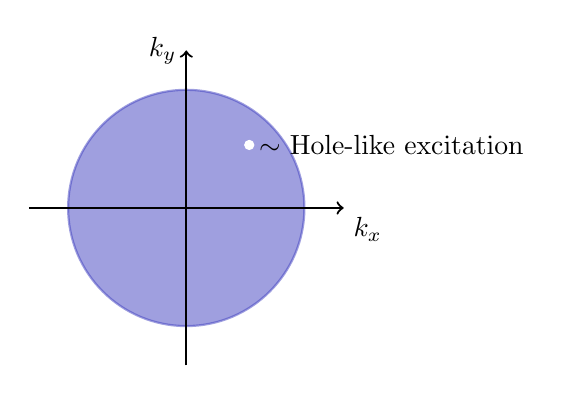
\begin{tikzpicture}[scale = 1]
	
	\coordinate (a) at (2, 2);
	\draw[thick,fill, blue!50!gray,  opacity =0.5] (a) circle (1.5);
	
	\draw[thick, ->] (0,2) to (4,2);
	\draw[thick, ->] (2,0) to (2,4);
	
	\node[anchor = north west] at (4, 2) {$k_x$};	
	
	\node[anchor = east] at (2, 4) {$k_y$};
	
	
	\coordinate (c) at (2.8, 2.8);
	\draw[thick, fill, white] (c) circle (0.05);
%	
%	\node[anchor = east] at (-0.5, 3.5) {$\ket{\Phi_0}$:};
	\node[anchor = west, align = right] at (c) {$\sim$ Hole-like excitation};
\end{tikzpicture}